\documentclass[tikz,border=2pt]{standalone}
\usepackage{amsmath}
\usetikzlibrary{arrows.meta}
\begin{document}
% M/G/1 queue under an N-policy with N = 4, lambda = 1, S = 0.5: one sample path of L(t).
% Server off: arrivals at 0.6, 1.5, 2.9, 4.0 raise L to N = 4; server on: departures every 0.5,
% arrivals at 4.7, 5.6, 6.2; the system is empty at 7.5 (expected build-up N/lambda = 4, T(4) = 4).
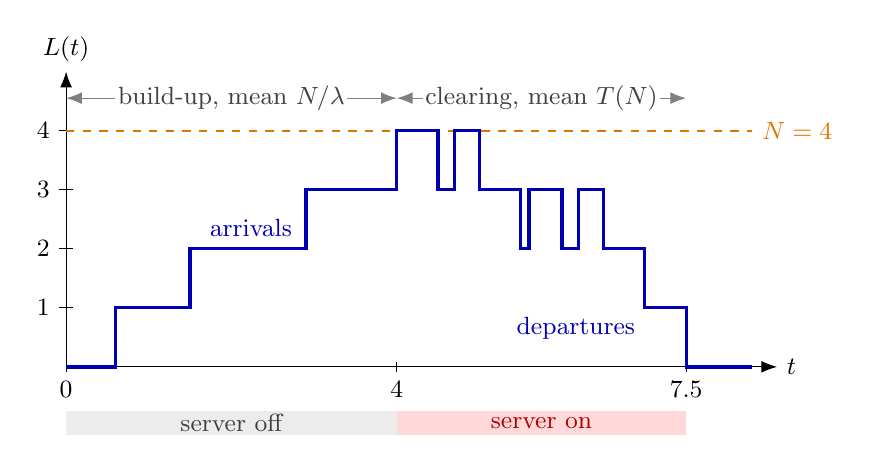
\begin{tikzpicture}[font=\small, >={Latex[length=2mm]}, x=1.05cm, y=0.75cm]
  % axes
  \draw[->] (0,0) -- (8.6,0) node[right] {$t$};
  \draw[->] (0,0) -- (0,5.0) node[above] {$L(t)$};
  \foreach \y in {1,2,3,4} \draw (0.08,\y) -- (-0.08,\y) node[left] {$\y$};
  \foreach \x/\lab in {0/0,4/4,7.5/7.5} \draw (\x,0.08) -- (\x,-0.08) node[below] {$\lab$};
  % threshold N
  \draw[orange!90!black, thick, dashed] (0,4) -- (8.3,4);
  \node[orange!90!black, anchor=west] at (8.3,4) {$N=4$};
  % phases
  \fill[gray!15] (0,-0.75) rectangle (4,-1.15);
  \fill[red!15] (4,-0.75) rectangle (7.5,-1.15);
  \node[gray!50!black] at (2,-0.95) {server off};
  \node[red!70!black] at (5.75,-0.95) {server on};
  \draw[<->, gray] (0,4.55) -- (4,4.55);
  \node[gray!50!black, fill=white, inner sep=1pt] at (2,4.55) {build-up, mean $N/\lambda$};
  \draw[<->, gray] (4,4.55) -- (7.5,4.55);
  \node[gray!50!black, fill=white, inner sep=1pt] at (5.75,4.55) {clearing, mean $T(N)$};
  % sample path
  \draw[blue!70!black, very thick] (0,0) -| (0.6,1) -| (1.5,2) -| (2.9,3) -| (4.0,4)
    -| (4.5,3) -| (4.7,4) -| (5.0,3) -| (5.5,2) -| (5.6,3) -| (6.0,2) -| (6.2,3)
    -| (6.5,2) -| (7.0,1) -| (7.5,0) -- (8.3,0);
  \node[blue!70!black, anchor=south east] at (2.85,2.05) {arrivals};
  \node[blue!70!black, anchor=north east] at (7.0,1) {departures};
\end{tikzpicture}
\end{document}
